\documentclass{article}

% if you need to pass options to natbib, use, e.g.:
% \PassOptionsToPackage{numbers, compress}{natbib}
% before loading nips_2018

% ready for submission
\usepackage{nips_2018}

% to compile a preprint version, e.g., for submission to arXiv, add
% add the [preprint] option:
% \usepackage[preprint]{nips_2018}

% to compile a camera-ready version, add the [final] option, e.g.:
% \usepackage[final]{nips_2018}

% to avoid loading the natbib package, add option nonatbib:
% \usepackage[nonatbib]{nips_2018}

\usepackage[utf8]{inputenc} % allow utf-8 input
\usepackage[T1]{fontenc}    % use 8-bit T1 fonts
\usepackage{hyperref}       % hyperlinks
\usepackage{url}            % simple URL typesetting
\usepackage{booktabs}       % professional-quality tables
\usepackage{amsfonts}       % blackboard math symbols
\usepackage{nicefrac}       % compact symbols for 1/2, etc.
\usepackage{microtype}      % microtypography
\usepackage{algorithm}      
\usepackage{algorithmic}      
\usepackage{listliketab}      
\usepackage{bm}      
\usepackage{amsmath}
\usepackage{makecell}
\usepackage{tabu}
\usepackage[table]{xcolor}
\usepackage{graphicx}
\usepackage{sidecap}


%\newcommand{\sym}[1]{\text{\sffamily \scshape #1}}
%\newcommand{\symx}{\text{\sffamily x}}
%\newcommand{\bW}{{\ensuremath{\bm{W}}}}
%\newcommand{\bU}{{\ensuremath{\bm{U}}}}
%\newcommand{\bh}{{\ensuremath{\bm{h}}}}
%\newcommand{\bb}{{\ensuremath{\bm{b}}}}
%\newcommand{\bq}{{\ensuremath{\bm{q}}}}
%\newcommand{\br}{{\ensuremath{\bm{r}}}}
%\newcommand{\bs}{{\ensuremath{\bm{s}}}}
%\newcommand{\bx}{{\ensuremath{\bm{x}}}}
%\newcommand{\ret}{{\ensuremath{\scriptscriptstyle R}}}
%\newcommand{\sto}{{\ensuremath{\scriptscriptstyle S}}}
%\newcommand{\evt}{{\ensuremath{\scriptscriptstyle Q}}}
%\newcommand{\tc}{{\ensuremath{\tilde{\tau}}}}
%\newcommand{\btau}{{\ensuremath{\bm{\tau}}}}
%\newcommand{\bM}{{\ensuremath{\hat{\bm{h}}}}}
%\newcommand{\TC}{{\ensuremath{\smash{\tilde{T}}}}}
\newcommand{\Win}{{\ensuremath{\bm{W}^{\textsc{in}}}}}
\newcommand{\vin}{{\ensuremath{\bm{v}^{\textsc{in}}}}}
\newcommand{\Wout}{{\ensuremath{\bm{W}^{\textsc{out}}}}}
\newcommand{\vout}{{\ensuremath{\bm{v}^{\textsc{out}}}}}
\newcommand{\fout}{{\ensuremath{f^{\textsc{out}}}}}
\newcommand{\cue}{{\ensuremath{\bm{c}}}}

% CITATIONS
%\citet{jon90}	    -->    	Jones et al. [21]
%\citet[chap. 2]{jon90}	    -->    	Jones et al. [21, chap. 2]
%\citep{jon90}	    -->    	[21]
%\citep[chap. 2]{jon90}	    -->    	[21, chap. 2]
%\citep[see][]{jon90}	    -->    	[see 21]
%\citep[see][chap. 2]{jon90}	    -->    	[see 21, chap. 2]
%\citep{jon90a,jon90b}	    -->    	[21, 32]



\title{State-Denoised Recurrent Neural Networks}

% The \author macro works with any number of authors. There are two
% commands used to separate the names and addresses of multiple
% authors: \And and \AND.
%
% Using \And between authors leaves it to LaTeX to determine where to
% break the lines. Using \AND forces a line break at that point. So,
% if LaTeX puts 3 of 4 authors names on the first line, and the last
% on the second line, try using \AND instead of \And before the third
% author name.


\author{
  Michael C.~Mozer\\
  Department of Computer Science\\
  University of Colorado\\
  Boulder, CO 80309\\
  \texttt{mozer@colorado.edu}\\
  \And
  Denis Kazakov\\
  Department of Computer Science\\
  University of Colorado\\
  Boulder, CO 80309\\
  \texttt{denis.kazakov@colorado.edu}\\
  %\And
  %Robert V.~Lindsey\\
  %Imagen Technologies\\
  %New York, NY\\
  %\texttt{lindsey@imagen.ai}\\
  %% Coauthor \\
  %% Affiliation \\
  %% Address \\
  %% \texttt{email} \\
  %% \And
  %% Coauthor \\
  %% Affiliation \\
  %% Address \\
  %% \texttt{email} \\
  %% \And
  %% Coauthor \\
  %% Affiliation \\
  %% Address \\
  %% \texttt{email} \\
}


\begin{document}
% \nipsfinalcopy is no longer used

\maketitle
\bibliographystyle{abbrvnat} % ADDED BY MIKE

\begin{abstract}
\end{abstract}

\section{Introduction}
Noise robustness is a fundamental challenge for every 
information processing system. A traditional approach to handling noise
is to design preprocessing stages that estimate and filter noise
from an input signal \citep{Boll1979}.
%https://ieeexplore.ieee.org/abstract/document/1163209/
More recently in machine learning, loss functions have been explored to achieve
invariance to task-irrelevant perturbations in the input
\citep{Simard1992,Zheng2016}.  Such methods are suitable for handling external
noise, but we argue in this article that \emph{internal} noise can be an even
greater challenge. To explain what we mean by internal noise, consider a
deep-net architecture in which representations are transformed
from one hidden layer to the next. To the degree that the network weights are
not precisely tuned to extract only critical features of the domain, irrelevant
features may be selected and have the potential to interfere with subsequent
processing.  Recurrent architectures are particularly fragile because
internal-state dynamics can amplify noise over the course of sequence
processing \citep{MathisMozer1995}. In this article, we propose a suppression
method that improves the generalization performance of deep nets.
We focus on recurrent nets, where the potential benefits are most significant.

Our approach draws inspiration from a notably robust and flexible information
processing system---the human brain.  Although the brain operates in an
unfathomably high-dimensional continuous state space, the (conscious) mind is
driven to categorize and to interpret the world via language.  We argue that
categorization and interpretation processes serve to suppress noise and
increase the reliability of behavior. Categorization treats instances that
vary in incidental ways as identical: a chair is something you can sit on
regardless of whether it is made of wood or metal. Language plays a similar
role in cognition.  For example, \citet{Witthoftetal2003} have demonstrated
that color terms of one's native language influence a perceptual-judgment
task---selecting a color patch that best matches a reference patch.  The
linguistic label assigned to a patch is the basis of matching, not the 
low-level perceptual data.

% Text i like that is just irrelevant
%
%What is striking about the brain is
%the following. It operates in an unfathomably high-dimensional continuous 
%state space with the capacity for massively parallel processing, yet the 
%(conscious) mind operates on categories and symbols and language, 
%with narrow bottlenecks in reasoning, planning, and decision making
%\cite{PashlerJohnston1998}.  We argue that cognitive limitations serve to
%suppress noise and therefore increase the reliability of behavior.
%
%; further, this influence is reduced by verbal interference (i.e., methods
%that reduce an individual's ability to use language). 
%Their experiments indicate that decision processes---here, selecting a color 
%patch that best  matches a reference patch---operates on representations that 
%perceptual but are modulated by linguistic categories.
%
%As one simple illustration, 
% color language terms influence color judgments, a result one would not expect unless (a) conscious states are interpretations, and (b) we can't directly access the low-level perceptual information for decision making.
%

Suppressing variability facilitates \emph{communication} in
information-processing systems. Whether we are talking about groups of humans,
regions within the brain, components of an articulated neural net
architecture, or layers of a feedforward network, in each case information must
be communicated from a \emph{sender} to a \emph{receiver}. To ensure that
the receiver interprets a message as intended, the sender should limit its
messages to a canonical form that the receiver has interpreted successfully 
in the past.  Language serves this role in inter-human communication. We 
explore noise suppression methods to serve this role in 
intra-network communication in deep-learning models.

% if space, nilgai example
% nilgai:  cow, horse, antelope -- indian animal

In the next section, we describe a recurrent neural network architecture for
cleaning up noisy representations---an \emph{attractor net}. We then propose
integrating attractor networks into deep networks, specifically
sequence-processing networks, for denoising internal states.  We present a
series of experiments on small-scale problems to illustrate the methodology and
analyze its benefits, followed by experiments on more naturalistic problems
which also show reliable and sometimes substantial benefits of denoising,
particularly in data-limited situations.

\section{Noise Suppression Via Attractor Dynamics}

The attractor nets we explore are discrete-time nonlinear dynamical systems.
Given a static $n$-dimensional input $\cue$, the network state at iteration
$k$, $\bm{a}_k$, is updated according to:
\begin{equation}
\bm{a}_{k} = f \left( \bm{W} \bm{a}_{k-1} + \cue \right) ,
\label{eq:att_dyn}
\end{equation}
where $f$ is a nonlinearity and $\bm{W}$ is a weight matrix.  Under certain
conditions on $f$ and $\bm{W}$, the state is guaranteed to converge to a
\emph{limit cycle} or \emph{fixed point}. A limit cycle of length $\lambda$
occurs if $\lim_{k\to\infty} \bm{a}_k = \bm{a}_{k+\lambda}$. A fixed point is
the special case of $\lambda=1$.

Attractor nets have a long history beginning with the work of
\cite{Hopfield1982} that was partly responsible for the 1980s wave of
excitement in neural networks.  Hopfield defined a mapping from network state,
$\bm{a}$, to scalar \emph{energy} values via an energy (or Lyapunov) function,
and showed that the dynamics of the net perform local energy minimization. The
shape of the energy landscape is determined by weights $\bm{W}$ and input
$\cue$ (Figure~\ref{fig:energy}a).  Hopfield's original work is based on
binary-valued neurons with asynchronous update, but since then similar results
have been obtained for certain nets with continuous-valued nonlinear neurons
acting in continuous \citep{Hopfield1984} or discrete time \citep{Koiran1994}.
\begin{figure}[bt]%[100]%[bt]
   \begin{center}
   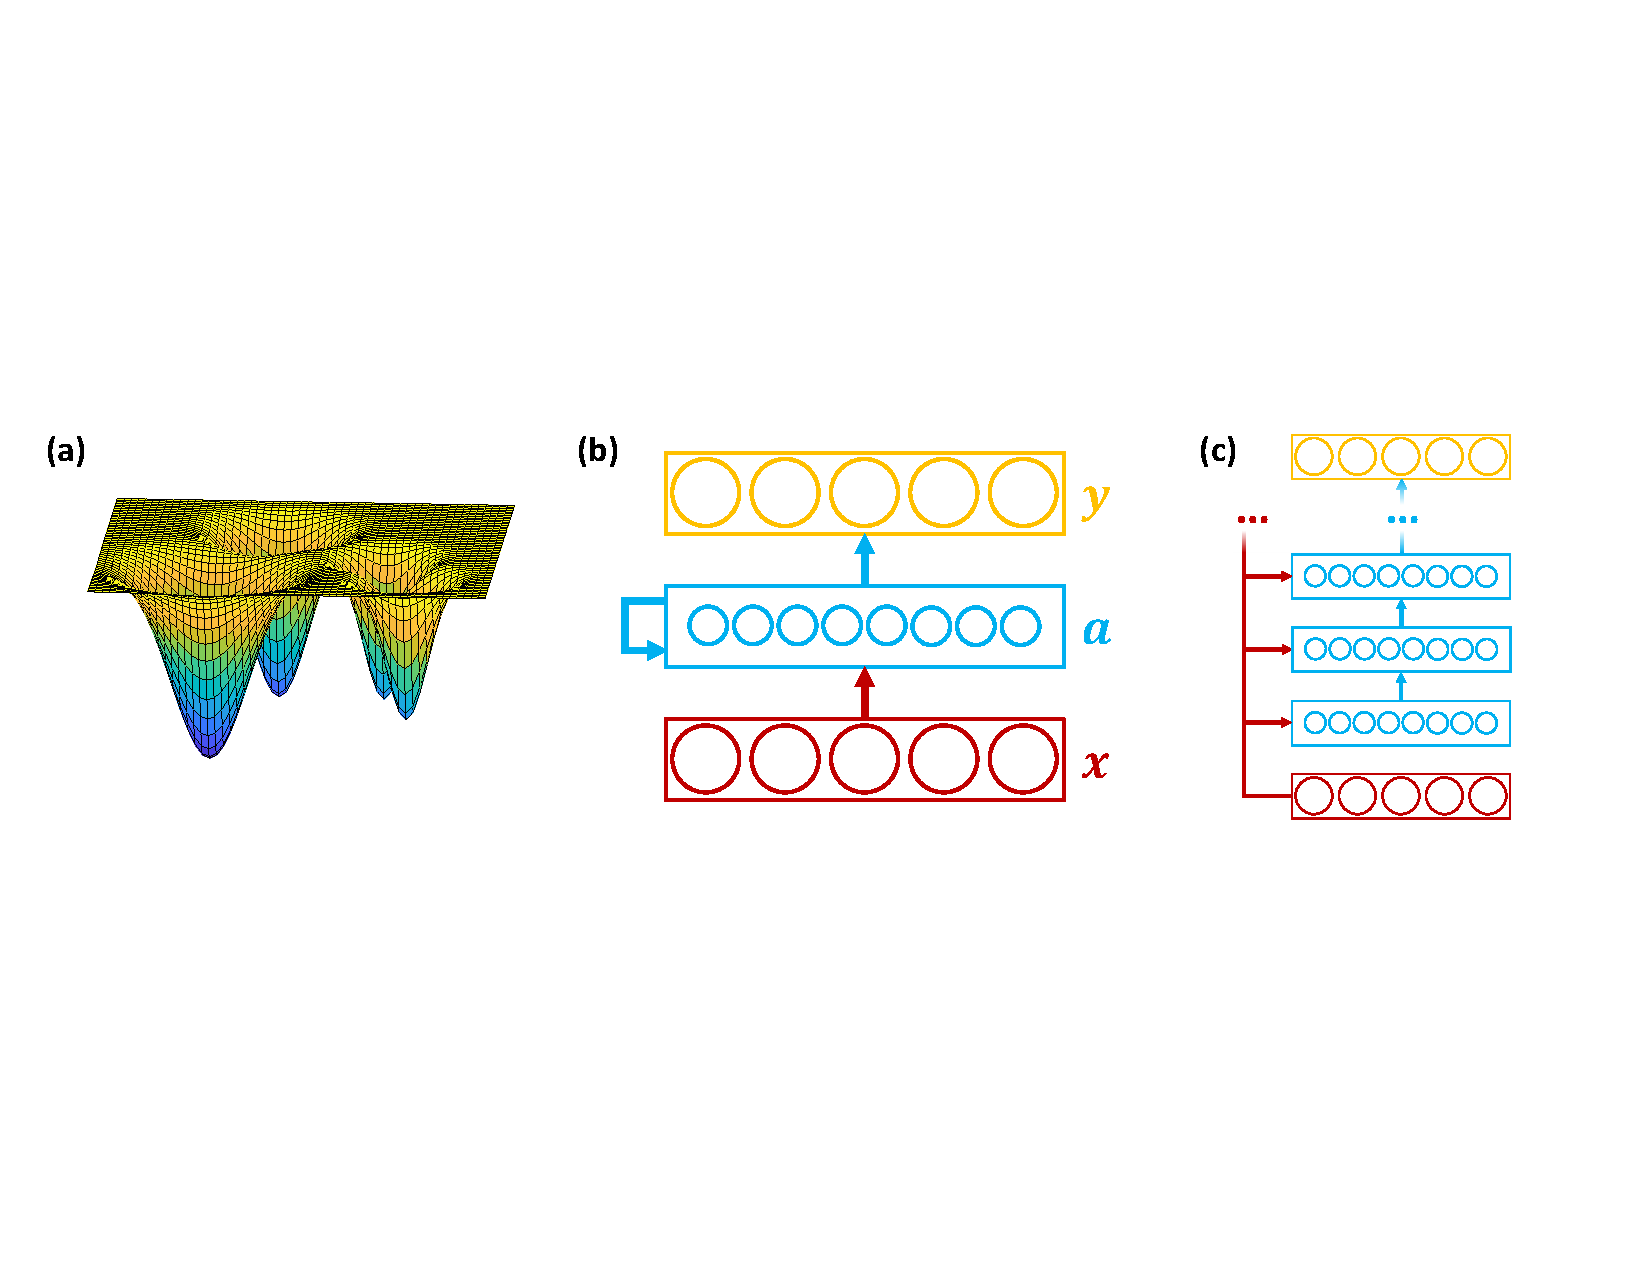
\includegraphics[width=5.5in]{fig/arch.pdf}
   \end{center}
   \caption{(a) energy landscape, (b) attractor net, (c) unfolded attractor net.}
   \label{fig:energy}
\end{figure}

We adopt Koiran's \citeyear{Koiran1994} framework, which dovetails with the
standard deep learning assumption of synchronous updates on continuous-valued
neurons. Koiran shows that with symmetric weights, $w_{ji} = w_{ij}$,
nonnegative self connections, $w_{ii} \ge 0$, and a bounded nonlinearity $f$
that is continuous and strictly increasing except at the extrema (e.g., tanh,
logistic, or their piecewise linear approximations), the network asymptotically
converges over iterations to a fixed point or limit cycle of length 2. As a 
shorthand, we refer to convergence in this manner as \emph{stability}.
%In practice, we almost always observe fixed point solutions.

Attractor nets have been used for multiple purposes, including
content-addressable memory, information retrieval, and constraint satisfaction
\citep{Mozer2009,Siegelmann2008}. In each application, the network is 
given an input containing partial or corrupted information, which we will refer
to as the \emph{cue}f denoted $\cue$; and the cue is mapped to
a canonical or \emph{well-formed} output in $\bm{a}_\infty$.
For example, to implement a content-addressible memory, a set of vectors, $\{
\bm{\xi}_1,\bm{\xi}_2,\ldots \}$, must first be stored. The energy landscape is
sculpted to make each $\bm{\xi}_i$ an attractor via a supervised training
procedure in which the target output is the vector $\bm{\xi}_i$ for some $i$
and the input is a noise-corrupted version of the target, e.g., $\cue =
\bm{\xi}_i \circ \bm{\eta}$, where $\circ$ denotes the Hadamard product and
$\eta_j \sim \mathrm{Bernoulli}(0.5)$. Following training, noise-corrupted
inputs should be `cleaned up' to reconstruct the state.

In the model we described, the attractor dynamics operate in the same
representational space as the input and output. Historically, this is the
common architecture. By projecting the input to a higher dimensional latent
space, we can design attractor nets with greater representational capacity.
Figure~\ref{fig:energy}b shows our architecture, with an
$m$-dimensional input, $\bm{x} \in [-1, +1]^m$, an $m$-dimensional output,
$\bm{y} \in [-1, +1]^m$, and an $n$-dimensional attractor state, $\bm{a}$,
where typically $n > m$ for representational flexibility.  The input $\bm{x}$
is projected to the attractor space via an affine transform:
\begin{equation}
\cue = \Win \bm{x} + \vin .  
\label{eq:cue} 
\end{equation} 
The attractor dynamics operate as in Equation~\ref{eq:att_dyn}, with
initialization $\bm{a}_0 = \bm{0}$ and $f \equiv \mathrm{tanh}$.  Finally, the
asymptotic attractor state is mapped to the output: 
\begin{equation} 
\bm{y} = \fout \left( \Wout \bm{a}_{\infty} + \vout \right) , 
\end{equation} 
where $\fout$ is an output activation function and the $\bm{W}^*$ and
$\bm{v}^*$ are free parameters of the model.

One way to conceptualize the operation of this network is that $\Win$ copies
the $m$ input features forward and the attractor net uses $m$ degrees of
freedom in its state representation to maintain these \emph{visible} features.
The other $n-m$ degrees of freedom can be used as \emph{latent} features that
impose higher-order constraints among the visible features (in much the same
manner as the hidden units in a restricted Boltzmann machine).  When the
attractor state is mapped to the output, $\Wout$ transfers just the visible
features.

As Equations~\ref{eq:att_dyn} and \ref{eq:cue} indicate, the input $\bm{x}$
biases the attractor state $\bm{a}_k$ at every iteration $k$, rather than---as
in the standard recurrent net architecture---being treated as an initial value,
e.g., $\bm{a}_0 = \bm{x}$. Effectively, there are short-circuit connections
between input and output to avoid vanishing gradients that arise in deep
networks (Figure~\ref{fig:energy}c). As a result of the connectivity, it is
trivial for the network to copy $\bm{x}$ to $\bm{y}$---and thus to propagate
gradients back from $\bm{y}$ to $\bm{x}$. For example, the network will
implement the mapping $\bm{y} = \bm{x}$ if: $m=n$, $\Win = \Wout  = I$, $\vin =
\vout = \bm{0}$, $\bm{W}=\bm{0}$, and $\fout$ is the identity mapping or an
identity mapping bounded at $-1$ and $+1$.

There is an alternative variation on the architecture that facilitates the pass
through of $\bm{x}$ to $\bm{y}$ which consists of: the input $\bm{x}$ in
Equation~\ref{eq:cue} being replaced with $\mathrm{tanh}^{-1}(\bm{x})$, $\fout
\equiv \mathrm{tanh}$, and the nonlinearity in the attractor dynamics 
shifted back one iteration, i.e., Equation~\ref{eq:att_dyn} becomes $\bm{a}_{k}
= \bm{W} f(\bm{a}_{k-1}) + \cue$. To ensure numerical stability, one can
treat the input as $\mathrm{tanh}^{-1}((1-\epsilon) \bm{x})$ for some small 
$\epsilon$.

\begin{figure}[bt]%[100]%[bt]
   \begin{center}
   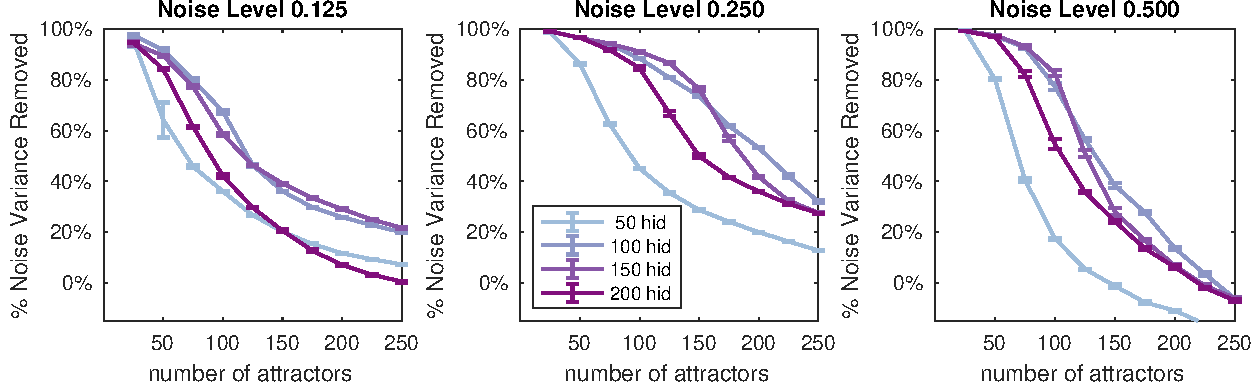
\includegraphics[width=5.5in]{fig/plot_attractor_performance.pdf}
   \end{center}
   \caption{Percentage noise variance suppression by an attractor net trained 
   on 3 noise levels. In each graph, the number of hidden units and number 
   of attractors to be learned is varied.  Evaluation is with 
   noise level 0.250, 50-dimensional inputs, and 10 replications. 
   Error bars indicate $\pm1$ SEM.}
   \label{fig:attractor_alone}
\end{figure}


\section{State-Denoised Recurrent Neural Networks}
L2 regularization of attractor weights 

for each minibatch, one update of the task weights, update the attractor weights for up to 10 steps until loss drops below 1.i


Training the attractor net:
and y as the target output
$x = s ( s^{-1}(y) + \eta )$ with $\eta \sim \mathcal{N}(0,\sigma^2)$.

how do we detect stability? $|\bm{a}_{k+2}-\bm{a}_k|_\infty < \theta$

\section{Simulations}

\subsection{Parity}

%notes:  10-long sequences
%train set = 1/4
%test set 1 = held out 3/4 without noise
%test set 2 = original train set with noise added (2 copies of each training example)
% 5000 epochs, batch training (to avoid random help of sgd)
% ADAM optimizer with default parameters
% lrate .008 on both prediction and attractor
% report test for best accuracy on train set
% no overfitting -- better train performance = better test performance

Task: length $L=10$ or $L=12$ bit sequences train on all $2^L$ sequences.  
It would be nice to have two testing sets:  (1) the same $2^L$ sequences 
with additional Gaussian noise added.  Choose noise level so that standard 
RNN is not at floor or ceiling in performance (e.g., ~75\% correct).
(2) longer noise-free sequences, of length $L+L\prime$, and chose $L\prime$
such that performance of the standard RNN is not at floor or ceiling.
Note that the performance levels you have in your results so far are TOO 
LOW. I expect that if you make the task a bit easier, you'll see more
difference between the different architectures.

Compare (a) basic tanh RNN, (b) RNN with attractor architecture,
single training objective, (c) RNN with attractor architecture, trained 
for noise robustness. Unless you have a better name, call these: RNN, ARNN
(attractor RNN), SDRNN (state denoised RNN).

100 replications. Compute Mean, median, std dev of generalization
performance. Perform t-tests to determine reliability.
Show separate results for the noisy sequences and the longer sequences.

NOTE: this simulation requires that you pick 4 model paramters:
elative learning rate for attractor dynamics, relative noise level in 
attractor training, and forgetting (L2 regularization) rate, and 
the dimensionality of the attractor space.  To tell a really nice story,
you'd have found the optimum by searching in this 4D parameter space, and
use this optimum for the basic parity simulation. Then for each of the
simulations below in which you manipulate one parameter at a time, you'd
freeze the other parameters to be the optima. Since it would be a huge
simulation to pick the conjunction of the 4 parameters optimally, it's
probably good enough for you to pick the parameters you expect to be best
based on your past simulations.

\subsubsection{Interpreting model}

Show that SDRNN has lower entropy than RNN. I'm not sure of the best
way to visualize. Try lots of things. You've made neat graphs showing entropy
reduction over the course of training, but this may be TMI for a paper or
talk. Perhaps just the entropy of the trained net, on both training and test
sets? 

For this simulation and the ones that follow, I can't say for sure that
we'll want to present results from both the training and test sets. I think we
need to make and see the figures to decide what we want to present and what
best conveys our conclusions from a simulation.

\subsubsection{Relative learning rate}
Explore relative learning rate for attractor dynamics: vary from 0 to
some upper bound. training and testing performance. 100 replications.

\subsubsection{Attractor basins}  
Vary noise level, which affects the size of the attractor basins.
Vary from 0 to some upper bound. training and testing performance. 100 
replications.

\subsubsection{Forgetting}  
Vary L2 weight decay of the recurrent attractor weights.
Vary from 0 to some upper bound. training and testing performance. 100 
replications.

\subsubsection{Attractor dimensionality}
Vary the number of units in the space where attractor dynamics are operating.
You may have a better name than "attractor dimensionality". Let's look
at training and testing performance. 100 replications.

\subsection{Majority task}

Figure out what length $L$ to use, train on a small subset of the sequences,
test on a large random subset. Compare the same 3 architectures: RNN,
ARNN, SDRNN. (Remember, please use TANH neurons, not GRU.) For this
simulation, we just need to compare generalization performance of the 3
models for a set of model parameters that you choose based on the parity
simulation.

\subsection{Simple finite-state machine}

Let's use the architecture I studied that seemed to get reasonable results.
If we want an alternative task, weould have a mult-class task which is
to count the length of the longest sequence of 1's in the input, with
all sequences having between 2 and 5. Maybe train on sequences of length
$L=15$ and a relatively small training set to make the task hard.

\subsection{Larger, Naturalistic Data Sets}

3-4 larger scale data sets: POS, Sentiment, Reuters Newswire topics classification, IMDB, etc.  You don't need to explore model parameters, but you could
use a validation set to pick the best SDRNN parameters. Don't cheat and pick
based on the test set.

\section{Relationship to Other Literature}


% Relation to theories of consciousness, Bengio's consciousness prior,
% and Andreas's learning with latent language, Ba's short-term memories
Varieties of consciousness:  access and phenomenal
degrees of consciousness

Global workspace (Dehaene 2017 article)

Conscious states are interpretations 
(Dehaene 
31. T. I. Panagiotaropoulos, G. Deco, V. Kapoor, N. K. Logothetis,
Neuron 74, 924–935 (2012).j
32. N. K. Logothetis, Philos. Trans. R. Soc. Lond. B Biol. Sci. 353,
1801–1818 (1998).

stability -- attractor states

Relationship to Ba's paper?
- symmetric update rule will lead to attractor dynamics
- learning within each sequence, vs. across sequences

http://www.offconvex.org/2018/02/17/generalization2/
- understanding deep nets in terms of noise suppression

A. Graves. “Adaptive Computation Time for Recurrent Neural Networks”, CoRR, Vol abs/1603.08983. 2016.

 \cite{AndreasKleinLevine2017}
 Learning with latent language -- assumes pretrained language interpretation
 module
 using the space of natural language strings as a parameter space is an effective way to capture natural task structure.



Relation to Bengio Consciousness prior
- proposal for a simplified or reduced description of an agent's complex, 
internal state that selectis a small subset of the information in the internal 
state, characterized in terms of factors, variables, concepts, dimensions
- emphasis on low dimensionality (e.g., key-value representation where only
one key is selected)
- instead, i focus on coherence of state such that all the bits fit together,
  but may involve multiple factors (e.g., dog -- hair, size, sound, etc.)
- bengio focus is on isolating factors; my goal is to build sharper internal
representations
- bengio's hope is to have a conscious state that can be transformed into
natural language sentences in a fairly simple manner.  in my case, it's more
of a criterion for what makes the conscious state.
- reduced states. us: interpretations. can be complex but packaged as atoms

Consciousness as a posterior: prior is bias to familiar states, interpretation
is posterior given evidence



%\begin{figure}[bt]%[100]%[bt]
%   \begin{center}
%   \includegraphics[width=4.25in]{fig/CTGRU.pdf}
%   \end{center}
%   \caption{A schematic of the GRU (left) and CT-GRU (right).
%   Color coding of the elements matches the background color used in the tables
%   presenting activation dynamics. For the CT-GRU, the large rectangle with
%   segments represents a multiscale hidden representation. The intrinsic decay
%   temporal decay of this representation, as well as the recurrent self-connections,
%   is not depicted in the schematic.}
%   \label{fig:CTGRU}
%\end{figure}
%\begin{SCfigure}[][b]
%   \includegraphics[width=4in]{fig/scaleMixture.pdf}
%   \caption{(a) Half life for a range of time scales: true value (dashed black line)
%   and mixture approximation (blue line). (b)
%   Decay curves for time scales $\tau \in [10, 100]$ (solid lines)
%   and the mixture approximation (dashed lines).
%   \label{fig:scaleMixture}}
%\end{SCfigure}
%
\newpage
\bibliography{references}

\end{document}

